\documentclass[12pt, titlepage]{report}
\usepackage[spanish]{babel}
\usepackage[none]{hyphenat} 
\usepackage[margin=3cm]{geometry}
\usepackage{graphicx}
\usepackage{subcaption}
\usepackage{parskip} 
\usepackage{longtable}
\usepackage{multirow, makecell}
\newcommand{\unit}[1]{\ensuremath{\, \mathrm{#1}}}
\usepackage{wrapfig}

\sloppy
\setlength{\parindent}{0cm}
\graphicspath{{img/}}
\renewcommand\thesection{\Alph{section}}
\renewcommand\thesubfigure{\Roman{subfigure}.}
\captionsetup[subfigure]{labelformat=simple}
\decimalpoint  

\begin{document}
    \begin{titlepage}
        \begin{center}
            \begin{figure}[ht]
                \centering
                \begin{subfigure}[r]{0.2\textwidth}
                    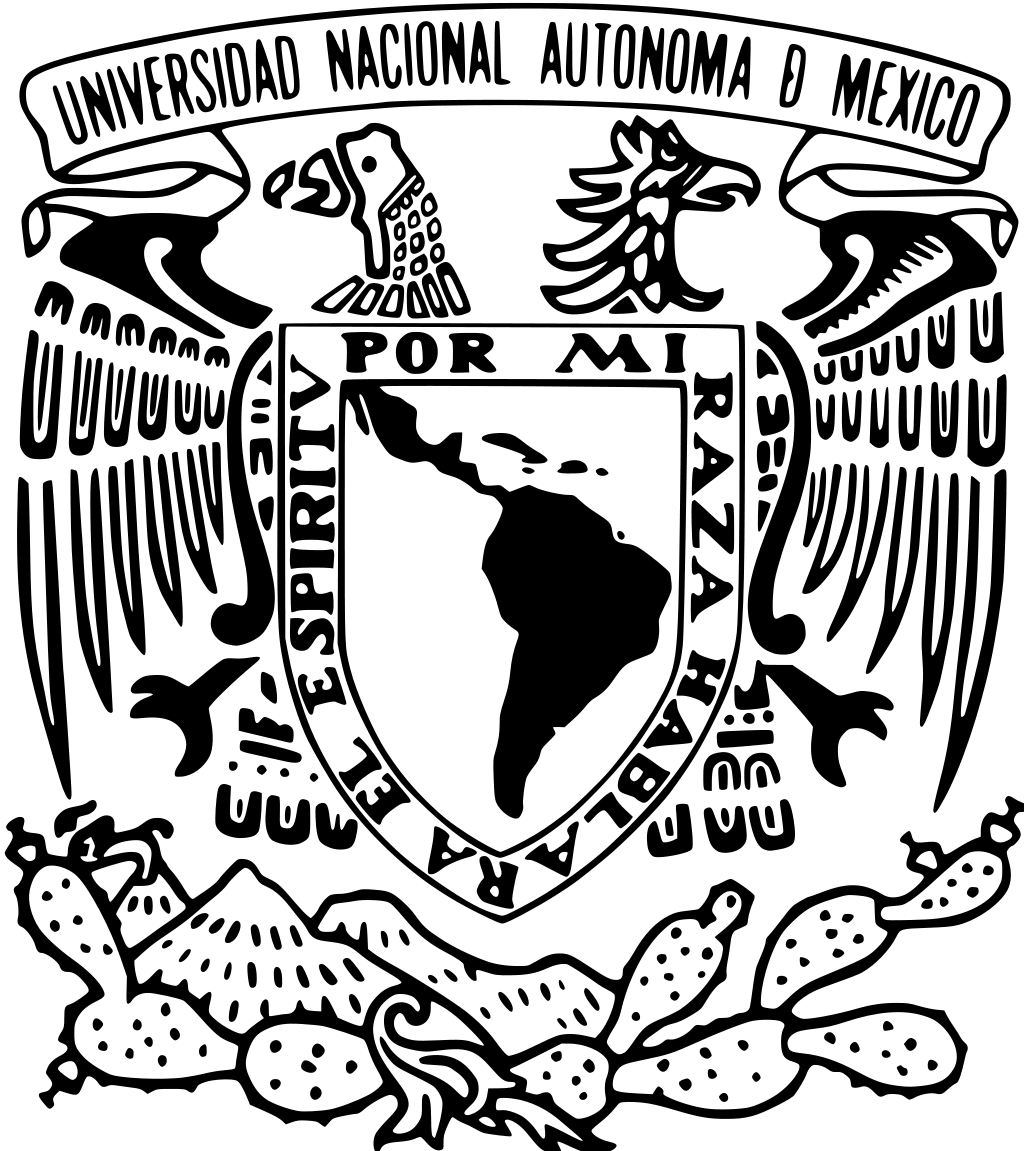
\includegraphics[width=\textwidth]{Escudo_UNAM.png}
                \end{subfigure} \hspace{9cm}
                \begin{subfigure}[l]{0.2\textwidth}
                    
\includegraphics[width=\textwidth]{Escudo_FI.png}
                \end{subfigure} 
            \end{figure}

            \Huge \textbf{\\Tercer examen parcial experimental\\}
            \huge Determinación experimental del centroide de un cuerpo\\
            \Huge \textbf{\\Mecánica\\}
            \huge \textbf{\\Nombre del profesor\\}
            \Large{Lorenzo O. Miranda Cordero\\}
            \huge \textbf{\\Nombre de los integrantes\\}
            \Large{Alan Omar Acosta Porcayo. No. lista 1\\Mauricio Gael Bonilla López. No. lista 9\\}
        \end{center}
    \end{titlepage}

    \section{Preparación de la tabla de madera}   
    \subsection*{Primer paso}
    La figura que se construyó para este proyecto consta de 4 figuras simples: un triángulo rectángulo, un cuadrado, un semicírculo hueco y un rectángulo hueco.

    \begin{figure}[ht]
        \centering
        \setcounter{figure}{0}
        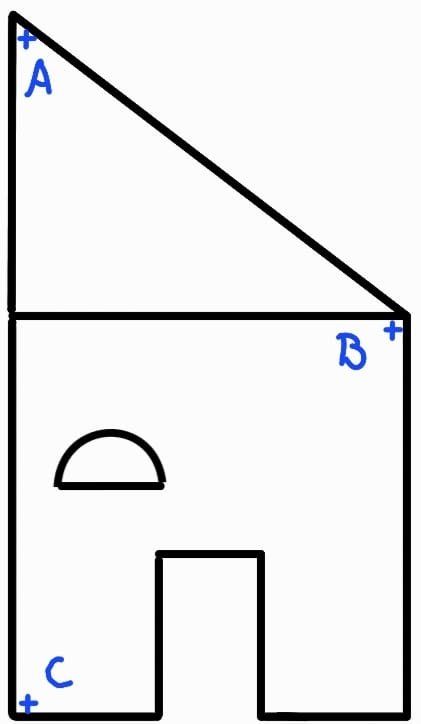
\includegraphics[width=2.5cm]{Croquis.jpg}
        \caption{Croquis con los puntos A, B y C}
    \end{figure}
    
    \begin{figure}[ht]
        \centering
        \begin{subfigure}{0.25\textwidth}
            \centering
            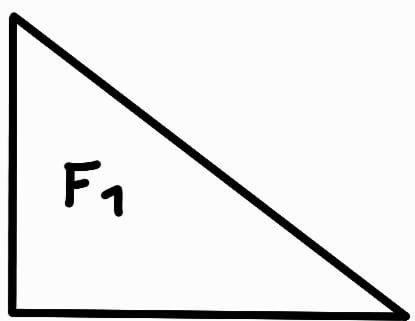
\includegraphics[width=2cm]{Croquis_Fig1.jpg}
            \caption{Triángulo\\rectángulo}
        \end{subfigure}  
        \begin{subfigure}{0.25\textwidth}
            \centering
            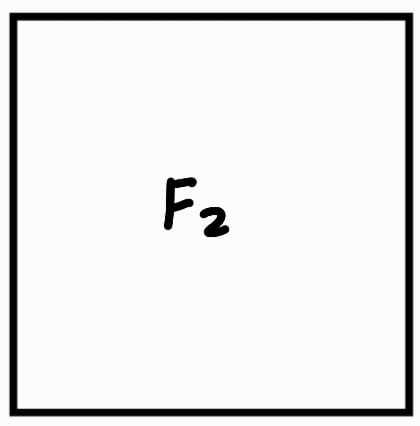
\includegraphics[width=2cm]{Croquis_Fig2.jpg}
            \caption{Cuadrado}
        \end{subfigure} 
        \begin{subfigure}{0.25\textwidth}
            \centering
            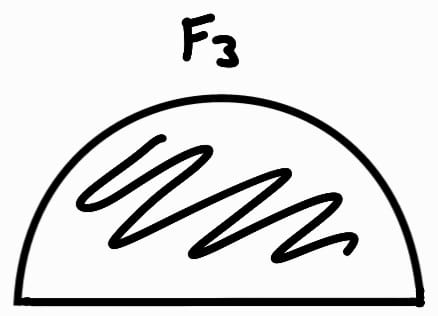
\includegraphics[width=2cm]{Croquis_Fig3.jpg}
            \caption{Semicírculo\\hueco}
        \end{subfigure} 
        \begin{subfigure}{0.25\textwidth}
            \centering
            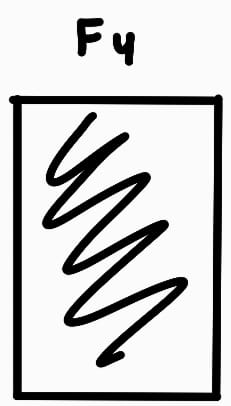
\includegraphics[width=1.5cm]{Croquis_Fig4.jpg}
            \caption{Rectángulo\\hueco}
        \end{subfigure}  
        \caption{Figuras simples}     
    \end{figure}

    Una vez realizado el croquis, en una hoja blanca tamaño carta se realizó el dibujo incluyendo las medidas que tendrá la tabla de madera.

    \begin{figure}[ht]
        \centering
        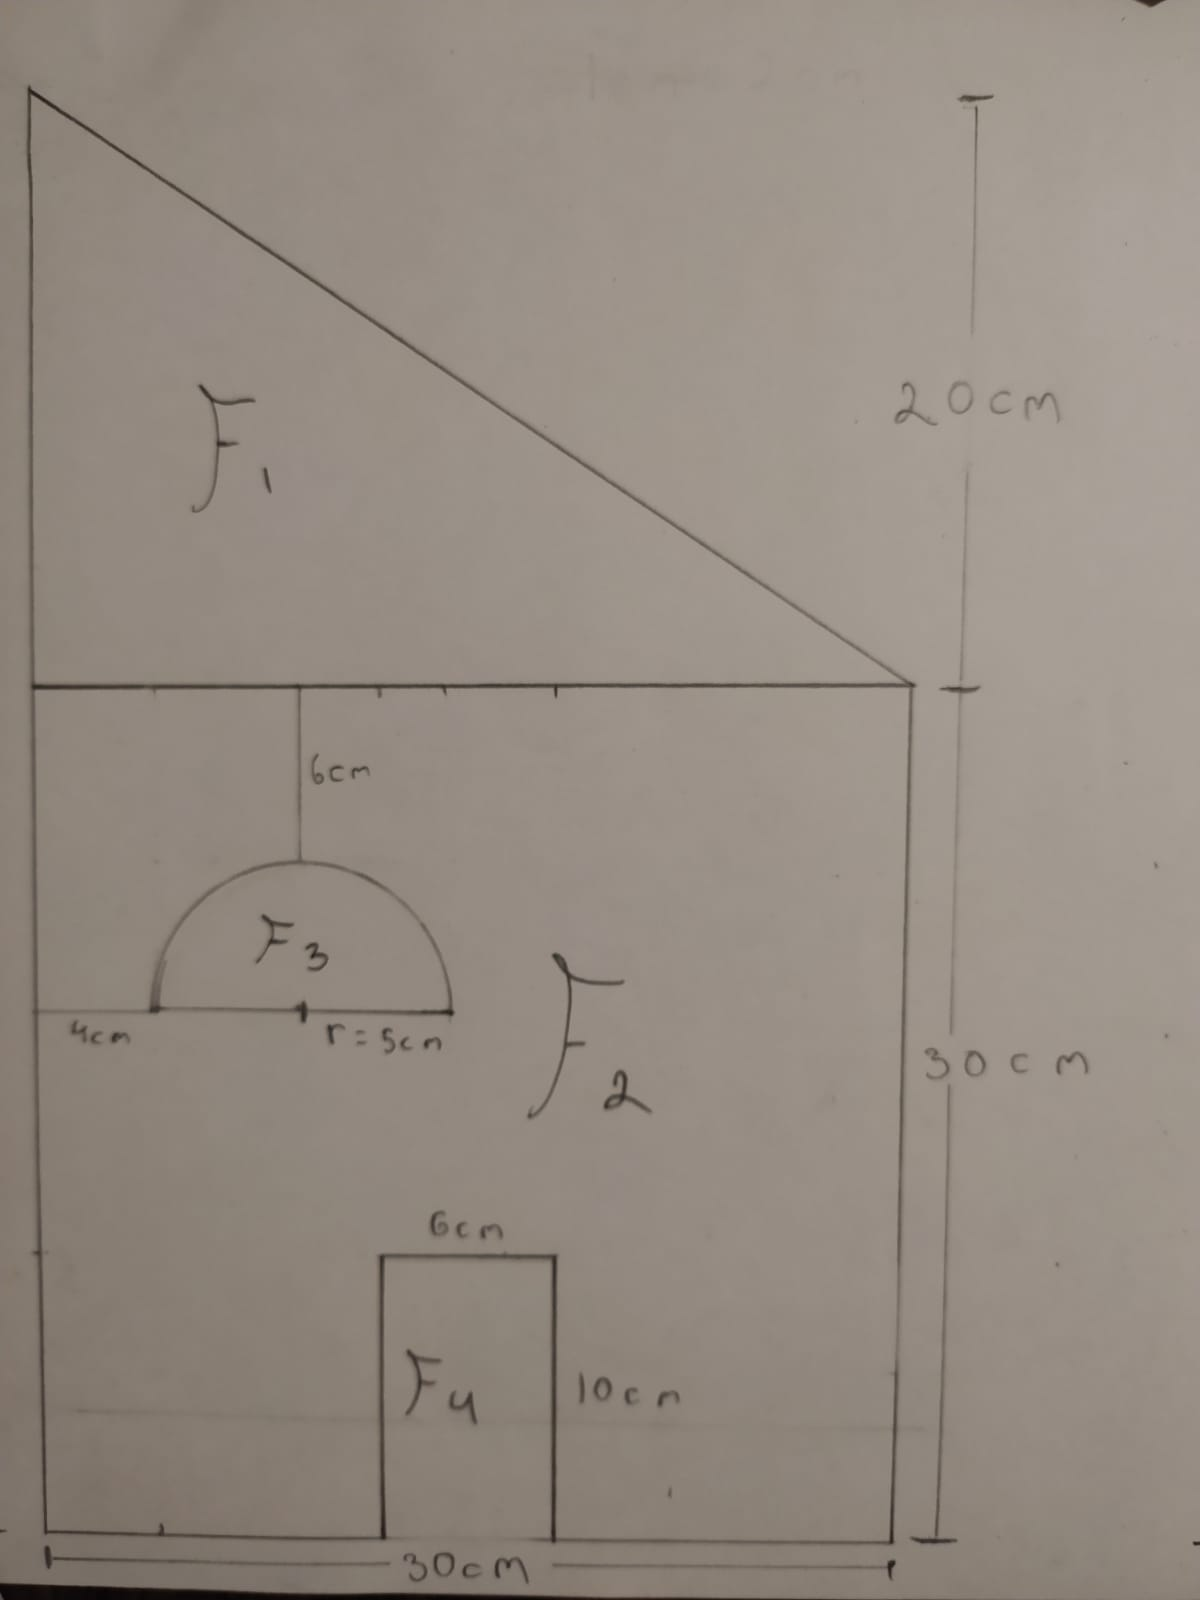
\includegraphics[width=0.5\textwidth]{Dibujo.jpg}
        \caption{Dibujo a escala numérica}
    \end{figure}

    \hfill
    \section{Modelación matemática de las fuerzas de los elementos elásticos (ligas o resortes) empleados}
    \subsection*{Segundo paso}
    Debido a que no contamos con un dinamómetro para medir las fuerzas utilizaremos tres ligas, las cuales caracterizaremos a partir de 5 pesas caseras creadas con bolsas de arroz previamente pesadas. Con la ayuda de estas mediciones obtendremos un modelo matemático para cada liga mediante un ajuste lineal.

    \begin{figure}[ht]
        \centering
        \begin{subfigure}[l]{0.4\textwidth}
            \centering
            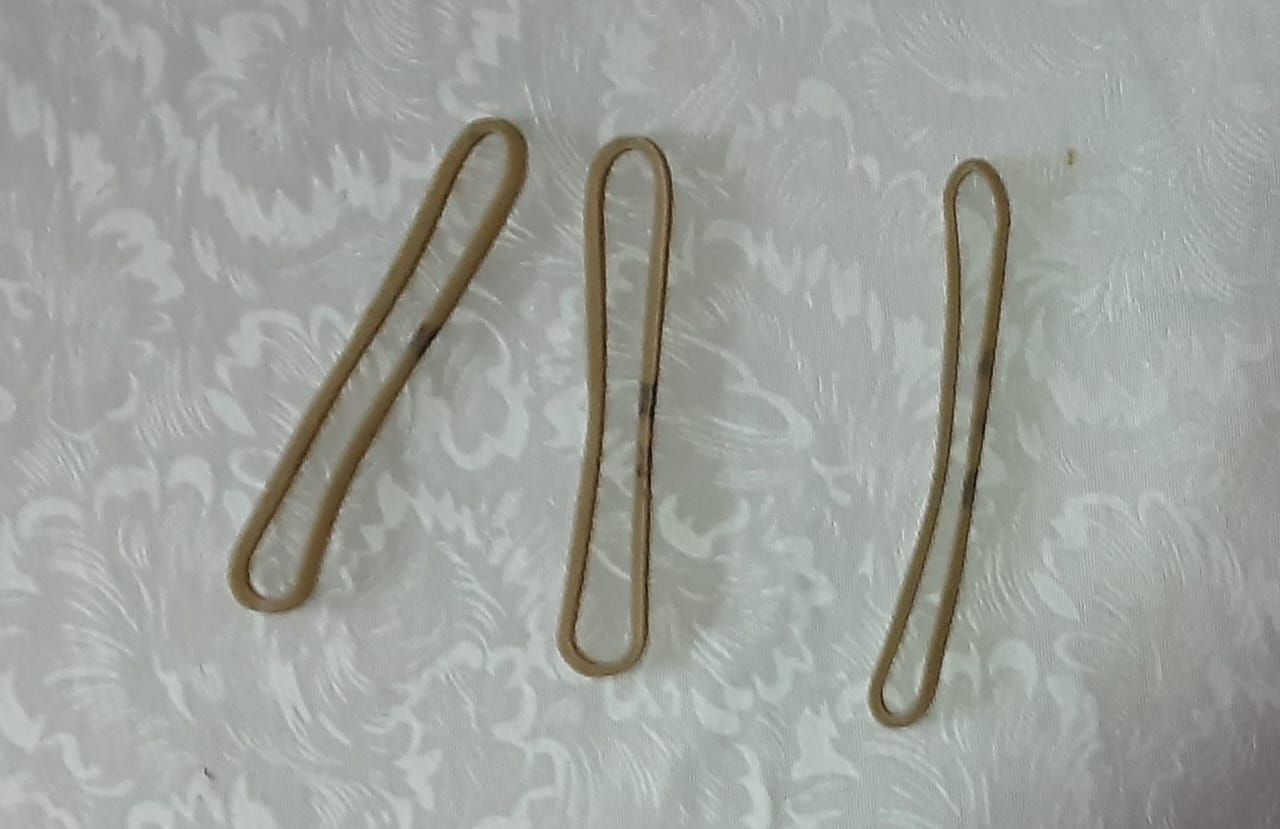
\includegraphics[height=3cm]{Ligas.jpg}
            \caption{Ligas}
        \end{subfigure}
        \begin{subfigure}[3]{0.4\textwidth}
            \centering
            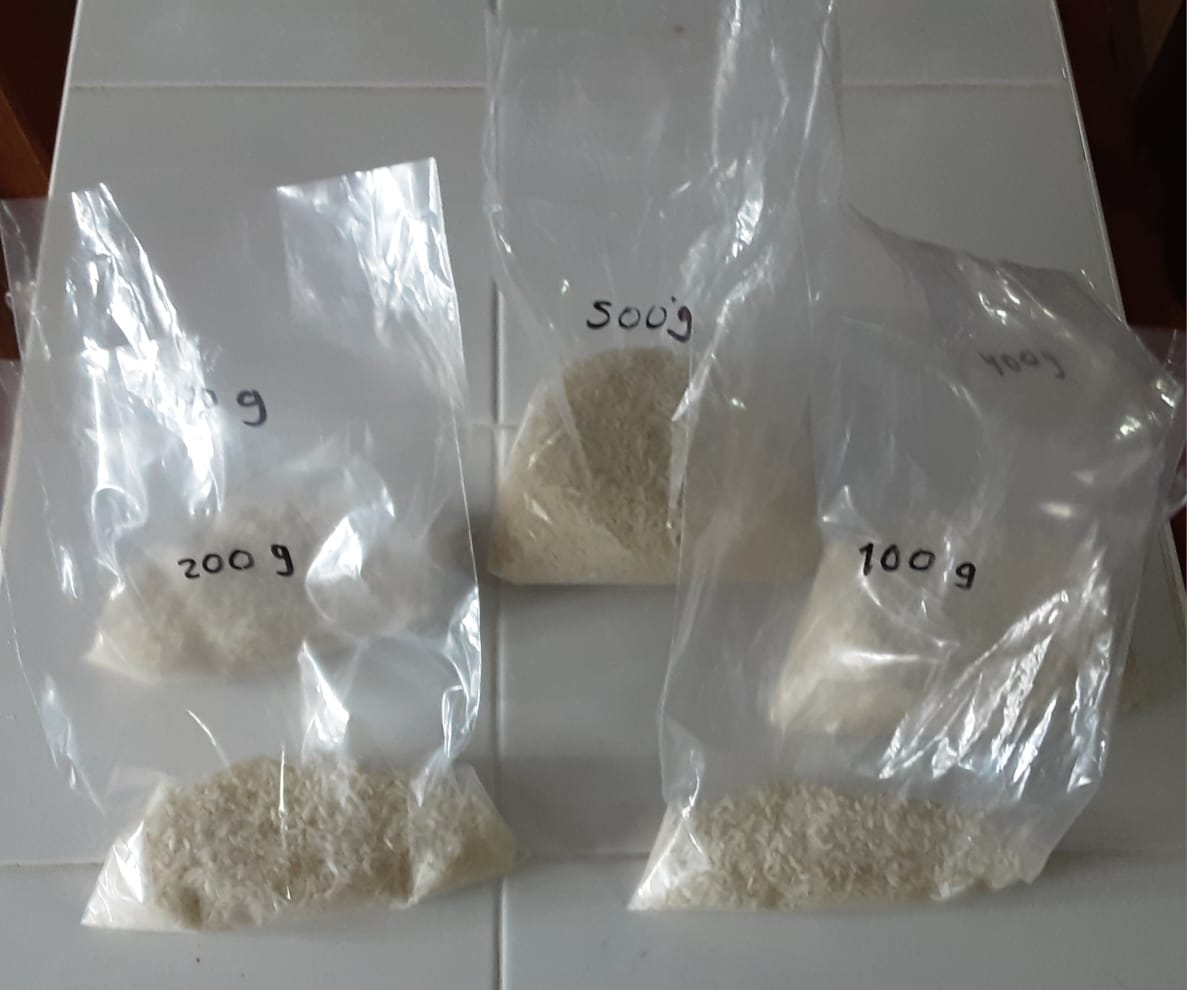
\includegraphics[height=3cm]{Pesas.jpg}
            \caption{Pesas}
        \end{subfigure}
        \caption{Materiales para medir fuerzas}
    \end{figure}

    \begin{longtable}{|c|c|c|}
        \hline
        \multicolumn{2}{|c|}{Masa} & \multirowcell{2}{Tensión \unit{[N]} \\ $m \unit{[kg]} \times 9.78 $} \\ \cline{1-2}
        [g] & [kg] & ~ \\ \hline
        100 & 0.1 & 0.978 \\ \hline
        200 & 0.2 & 1.956 \\ \hline
        300 & 0.3 & 2.934 \\ \hline
        400 & 0.4 & 3.912 \\ \hline
        500 & 0.5 & 4.890 \\ \hline
        \caption{Conversión de masa a fuerza}
    \end{longtable} 

    \subsection*{Tercer paso}
    Para el proceso de caracterización de cada liga se mide primero la longitud natural, es decir, sin aplicarle ninguna fuerza, registrando las mediciones en cm. Posteriormente, se utilizara cada peso para sujetarlo con la liga y medir la deformación de esta, anotando cada medición en una tabla.

    \begin{longtable}{|c|c|c|}
        \hline
        \multicolumn{3}{|c|}{Longitud natural (Ln) [cm] = 7.8 [cm]} \\ \hline
        Tensión (T) [N] & Longitud final (Lf) [cm] & Deformación $\delta$  (Lf $-$ Ln) [cm] \\ \hline
        0.978 & 8.5 & 0.7 \\ \hline
        1.956 & 9.3 & 1.5 \\ \hline
        2.934 & 10.3 & 2.5 \\ \hline
        3.912 & 12 & 4.2 \\ \hline
        4.890 & 13.5 & 5.7 \\ \hline
        \caption{Caracterización liga 1}
    \end{longtable}

    \begin{longtable}{|c|c|c|}
        \hline
        \multicolumn{3}{|c|}{Longitud natural (Ln) [cm] = 7.5 [cm]} \\ \hline
        Tensión (T) [N] & Longitud final (Lf) [cm] & Deformación $\delta$  (Lf $-$ Ln) [cm] \\ \hline
        0.978 & 8.4 & 0.9 \\ \hline
        1.956 & 9.1 & 1.6 \\ \hline
        2.934 & 10.5 & 3\\ \hline
        3.912 & 11.8 & 4.3 \\ \hline
        4.890 & 14 & 6.5 \\ \hline
        \caption{Caracterización liga 2}
    \end{longtable}

    \newpage
    \begin{longtable}{|c|c|c|}
        \hline
        \multicolumn{3}{|c|}{Longitud natural (Ln) [cm] = 8 [cm]} \\ \hline
        Tensión (T) [N] & Longitud final (Lf) [cm] & Deformación $\delta$  (Lf $-$ Ln) [cm] \\ \hline
        0.978 & 8.7 & 0.7 \\ \hline
        1.956 & 10 & 2 \\ \hline
        2.934 & 12 & 4 \\ \hline
        3.912 & 14.5 & 6.5 \\ \hline
        4.890 & 17 & 9 \\ \hline
        \caption{Caracterización liga 3}
    \end{longtable}

    \subsection*{Cuarto paso}
    Con base en los datos obtenidos para liga, se creó con ayuda de EXCEL una gráfica de F vs $\delta$ y se realizó un ajuste lineal que permite conocer la fuerza en el elemento elástico. El modelo matemático que se obtiene de cada gráfica tiene la siguiente forma: 
    $$T_1=k_1\delta+To_1$$
    $T_1= $ tensión en la liga 1 \\
    $k_1= $ constante de la liga 1 (pendiente de la recta) \\
    $\delta= $ deformación de la liga \\
    $To_1= $ fuerza residual en la liga (ordenada al origen)\\

    Los modelos matemáticos de cada liga son los siguientes:
    $$T_1 = 0.7533\delta + 0.7343 \unit{[N]}$$
    $$T_2 = 0.6807\delta + 0.715 \unit{[N]}$$
    $$T_3 = 0.4568\delta + 0.9057 \unit{[N]}$$

    \begin{figure}[ht]
        \centering
        \begin{minipage}[c]{0.45\linewidth}
            \centering
            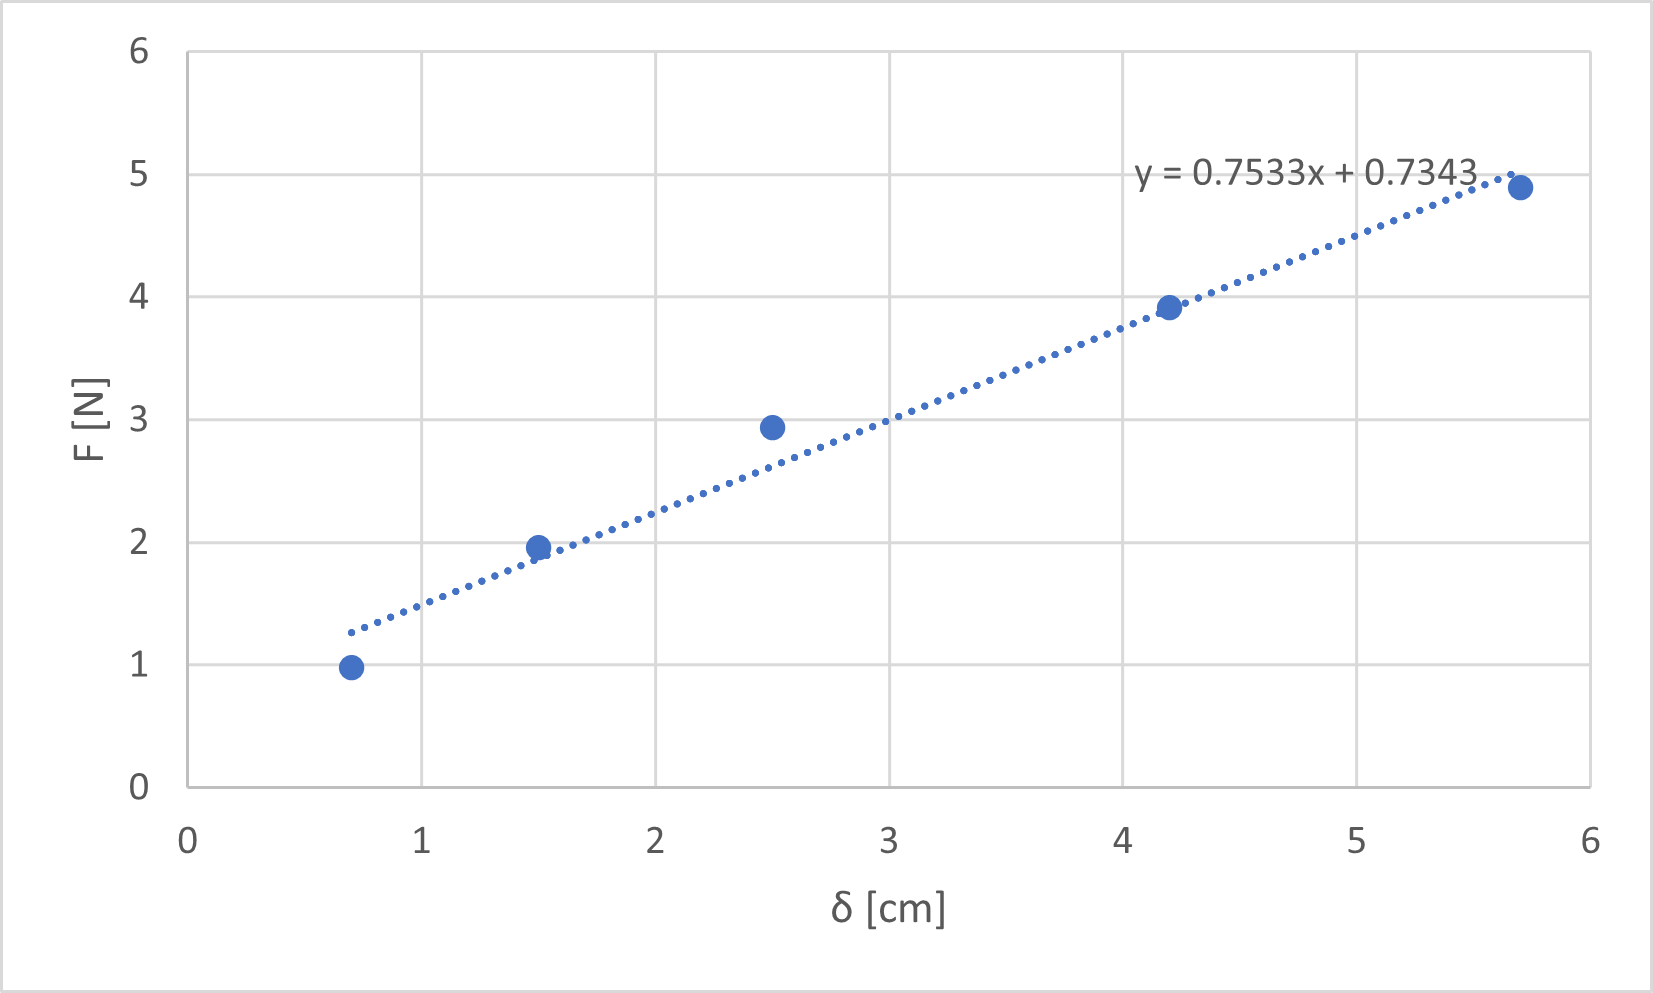
\includegraphics[width=7cm]{Graf1.png}
            \caption{Gráfica liga 1}
        \end{minipage}
        \begin{minipage}[c]{0.45\linewidth}
            \centering
            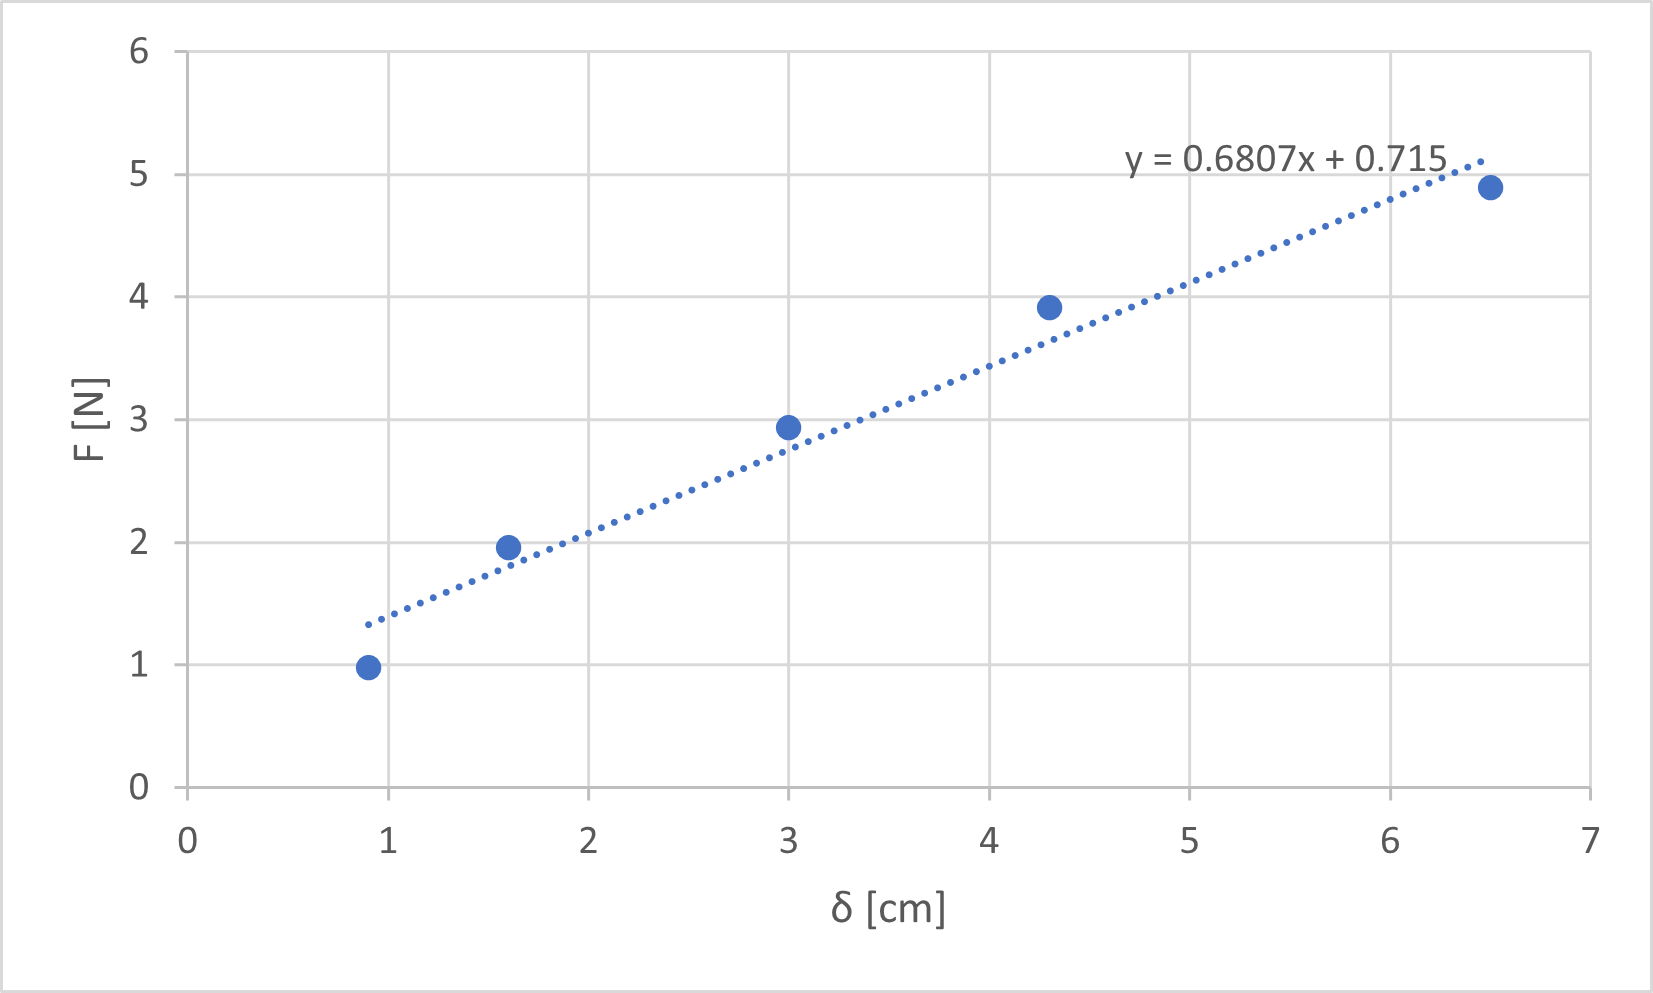
\includegraphics[width=7cm]{Graf2.png}
            \caption{Gráfica liga 2}   
        \end{minipage}
        \par\bigskip
        \begin{minipage}[c]{0.45\linewidth}
            \centering
            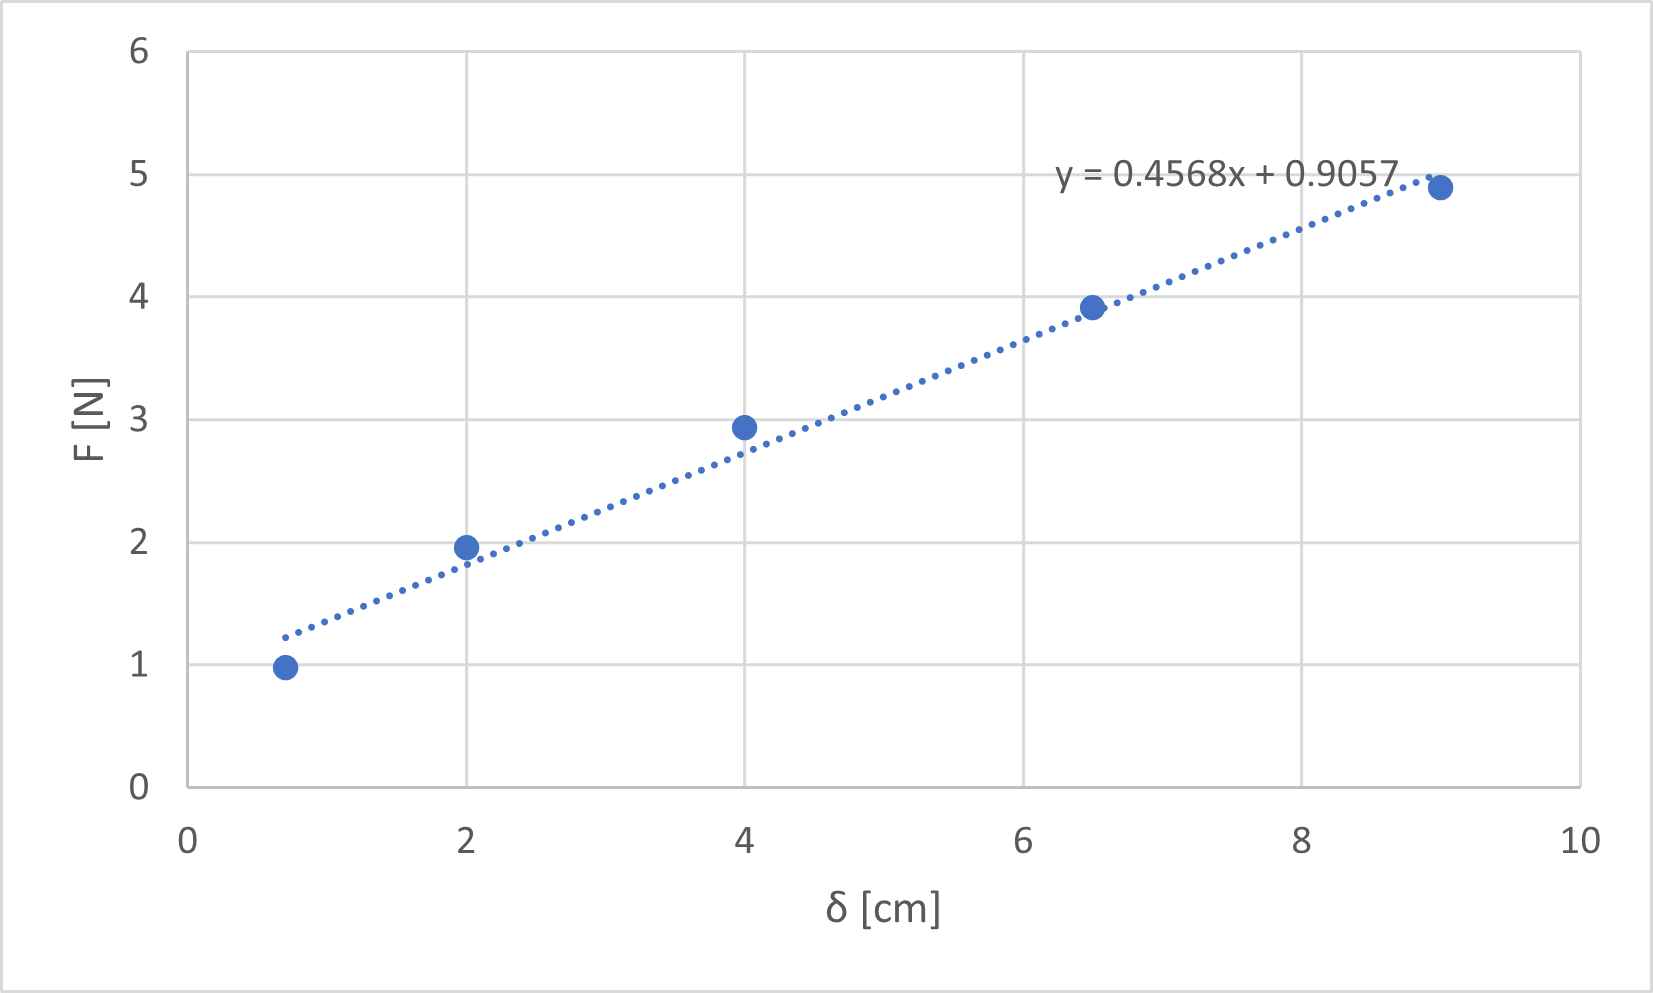
\includegraphics[width=7cm]{Graf3.png}
            \caption{Gráfica liga 3}
        \end{minipage}
    \end{figure}
    
    \newpage
    \subsection*{Quinto paso}
    El quinto paso consta de hacer el tercer y cuarto paso para las dos ligas restantes. La tabla, la grafica y el modelo matemático de cada liga se encuentra en la sección pertinente. 

    \hfill
    \section{Obtención en forma teórica del centroide ``C'' de la figura compuesta}
    \subsection*{Sexto paso}
    Al dibujo realizado en el primer paso se le colocó un sistema coordenado X$-$Y, y a partir de este sistema se obtienen las coordenadas del centroide en la figura plana, empleando las siguientes expresiones:
    $$\bar{X}=\frac{\sum_{i= 1}^{n} x_{i}A_{i}}{\sum_{i= 1}^{n}A_{i}}$$
    $$\bar{Y}=\frac{\sum_{i= 1}^{n} y_{i}A_{i}}{\sum_{i= 1}^{n}A_{i}}$$

    Figura 1:
    $$A_{1}=\frac{(30)(20)}{2}=300 \unit{[cm^2]}$$
    $$x_{1}=\frac{30}{3}=10 \unit{[cm]}$$
    $$y_{1}=30+\frac{20}{3}=36.66 \unit{[cm]}$$
    Figura 2:
    $$A_{2}=(30)(30)=900\unit{[cm^2]}$$
    $$x_{2}=\frac{30}{2}=15 \unit{[cm]}$$
    $$y_{2}=\frac{30}{2}=15 \unit{[cm]}$$
    Figura 3:
    $$A_{3}=-\frac{\pi(5^2)}{2}=-39.27\unit{[cm^2]}$$
    $$x_{3}=4+5=9 \unit{[cm]}$$
    $$y_{3}=19+\frac{4(5)}{3\pi}=21.12 \unit{[cm]}$$
    Figura 4:
    $$A_{4}=-(6)(10)=-60\unit{[cm^2]}$$
    $$x_{4}=12+\frac{6}{2}=15 \unit{[cm]}$$
    $$y_{4}=\frac{10}{2}=5 \unit{[cm]}$$
    
    $$ \bar{X}=\frac{\sum_{i= 1}^{n} x_{i}A_{i}}{\sum_{i= 1}^{n}A_{i}} = \frac{(10)(300)+(15)(900)+(9)(-39.27)+(15)(-60)}{300+900-39.27-60}$$
    $$ \bar{X}=\frac{3000+13500-353.43-900}{1100.73}=\frac{15246.57}{1100.73}= 13.85 \unit{[cm]}$$
    
    $$ \bar{Y}=\frac{\sum_{i= 1}^{n} y_{i}A_{i}}{\sum_{i= 1}^{n}A_{i}} = \frac{(36.66)(300)+(15)(900)+(21.12)(-39.27)+(5)(-60)}{300+900-39.27-60}$$
    $$ \bar{Y}=\frac{10998+13500-829.38-300}{1100.73}=\frac{23368.62}{1100.73}=21.23 \unit{[cm]}$$

    $$C(13.85, 21.23) \unit{[cm]}$$

    \subsection*{Séptimo paso}
    Una vez obtenidas las coordenadas del centroide ``C'', es posible marcar en la tabla de madera la posición de este centroide y, con ayuda de un soporte colocado en el centroide, lograr mantener la tabla en equilibrio.

    \begin{figure}[ht]
        \centering
        \begin{subfigure}[l]{0.4\textwidth}
            \centering
            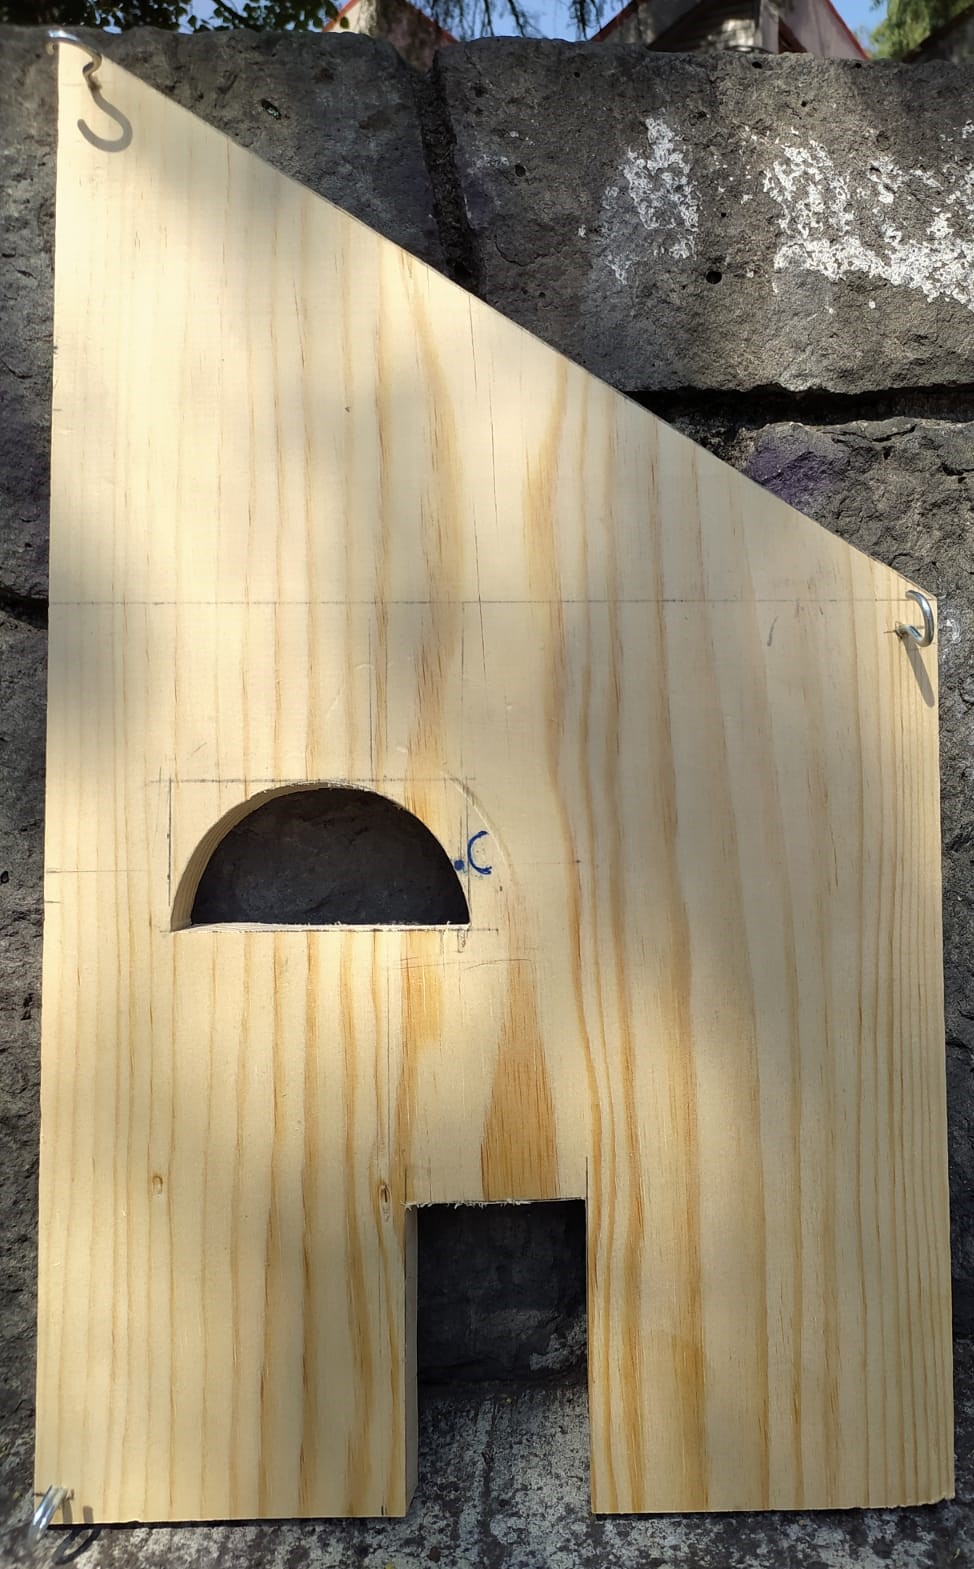
\includegraphics[height=6cm]{Centroide.jpg}
            \caption{Centroide marcado en la tabla}
        \end{subfigure}
        \begin{subfigure}[3]{0.4\textwidth}
            \centering
            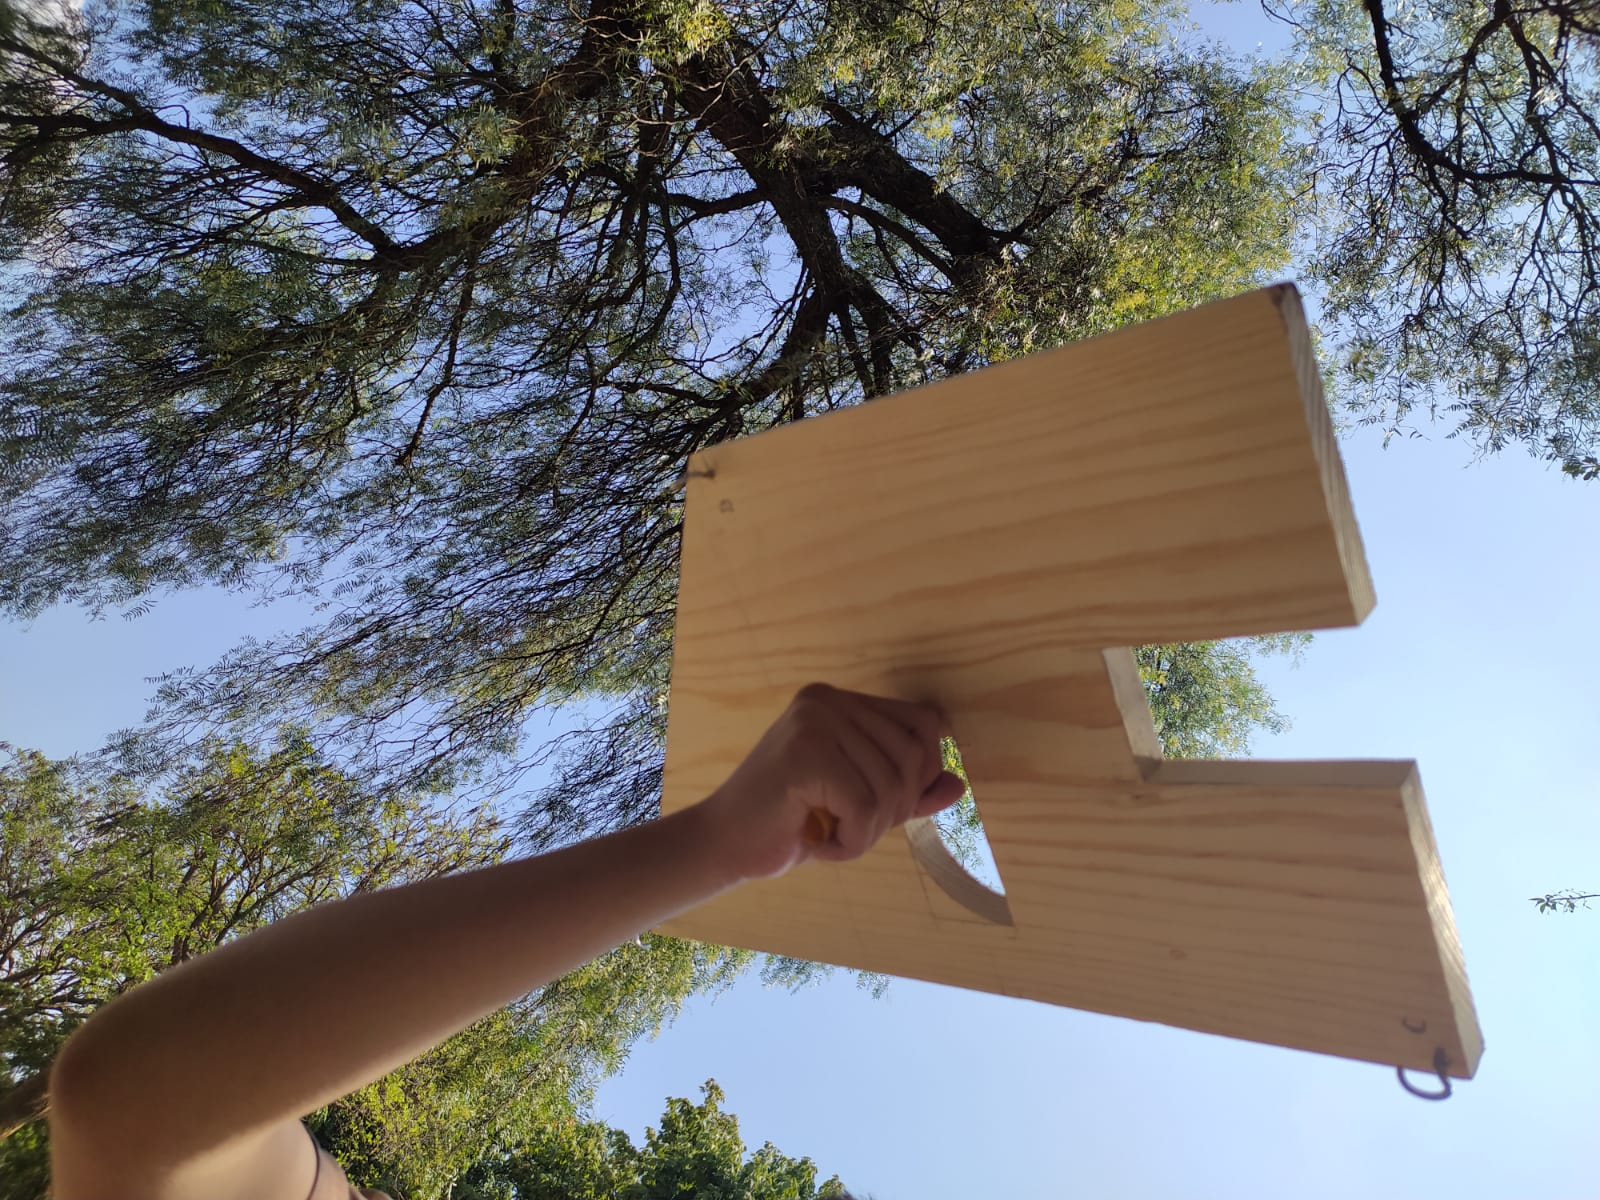
\includegraphics[width=6cm]{Equilibrio1.jpg}
            \caption{Tabla en equilibrio}
        \end{subfigure}
        \caption{Centroide en la tabla}
    \end{figure}

    \section{Elaboración de la tabla que se usará en el experimento}
    \subsection*{Octavo paso}
    A partir de la figura compuesta se cortó una pieza de madera de triplay con 18 mm de grosor, la cual fue hecha en una carpintería.

    \hfill
    \section{Registro de las tensiones que sostienen a la tabla}
    \subsection*{Noveno paso}
    A la tabla de madera se le colocaron tres armellas en los puntos A, B y C, que de acuerdo a nuestro sistema coordenado tienen las siguientes coordenadas:
    $$A(1, 48) \unit{[cm]}$$
    $$B(29, 29) \unit{[cm]}$$
    $$C(0.8, 1) \unit{[cm]}$$

    \subsection*{Décimo paso}
    La tensión de cada liga se calcula obteniendo primer la deformación que tiene al soportar el peso de la tabla y sustituyendo la deformación en su respectivo modelo matemático. 

    \begin{figure}[ht]
        \centering
        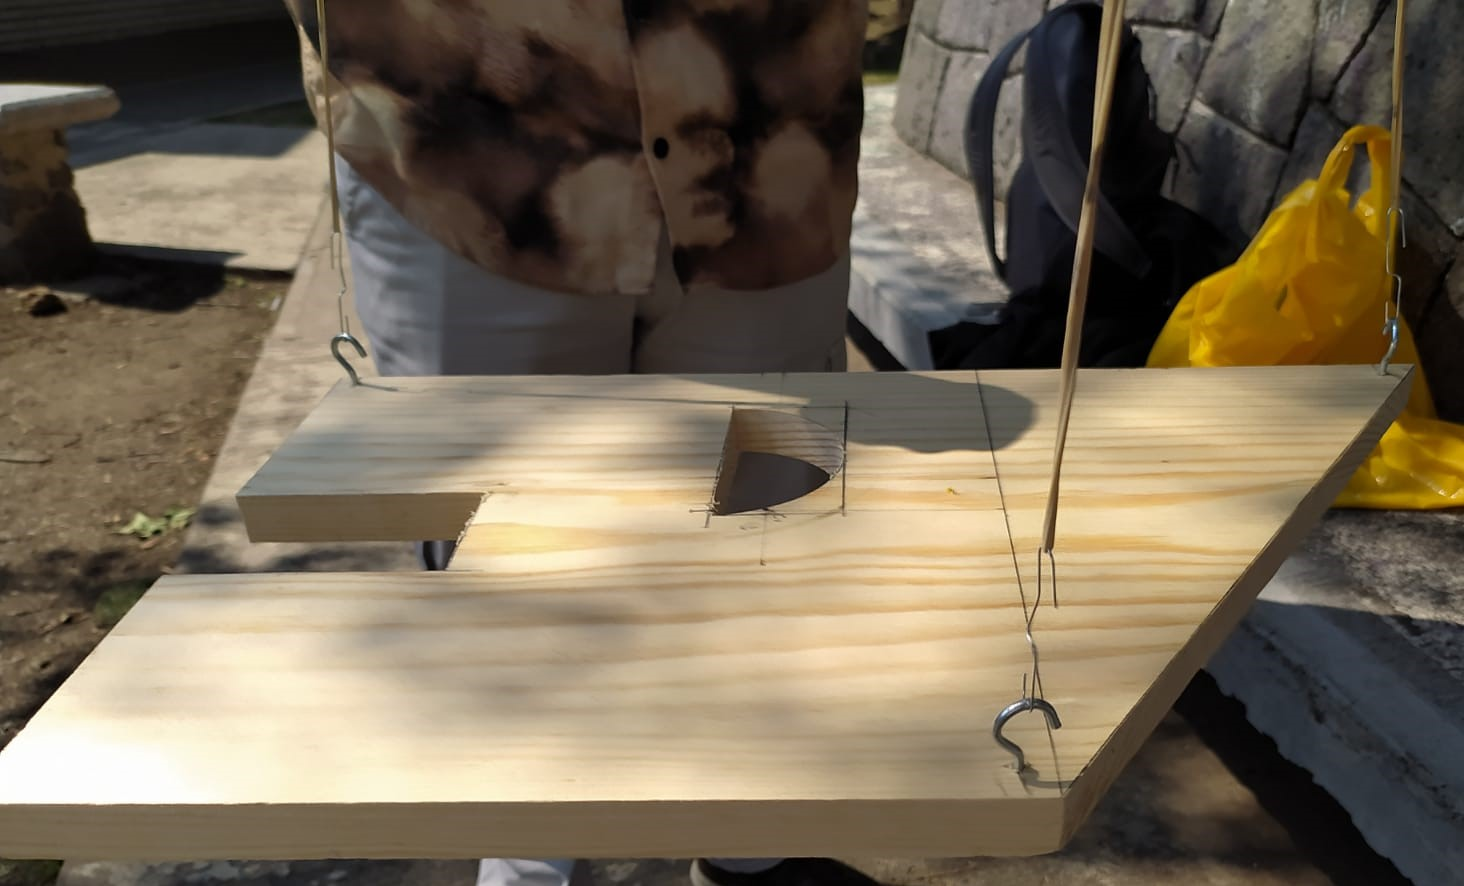
\includegraphics[width=0.5\textwidth]{Medicion.jpg}
        \caption{Medición de deformaciones}
    \end{figure}

    $$\delta_1=Lf_1-Ln_1= 9 - 7.8 \unit{[cm]} = 1.2 \unit{[cm]}$$
    $$\delta_2=Lf_2-Ln_2= 16 - 7.5 \unit{[cm]} = 8.5 \unit{[cm]}$$
    $$\delta_3=Lf_3-Ln_3= 16.5 - 8 \unit{[cm]} = 8.5 \unit{[cm]}$$

    $$T_1 = 0.7533\delta_1 + 0.7343 \unit{[N]} = 0.7533(1.2) + 0.7343 \unit{[N]} = 1.6383 \unit{[N]}$$
    $$T_2 = 0.6807\delta_2 + 0.715 \unit{[N]} = 0.6807(8.5)+ 0.715 \unit{[N]} = 6.5001 \unit{[N]}$$
    $$T_3 = 0.4568\delta_3 + 0.9057 \unit{[N]} = 0.4568(8.5) + 0.9057 \unit{[N]} = 4.7885 \unit{[N]}$$

    \hfill
    \section{Determinación del centro de gravedad ``G'' de la tabla con base en las tensiones obtenidas experimentalmente}
    \subsection*{Décimo primer paso}
    Una vez obtenidos $T_{1}$, $T_{2}$ y $T_{1}$, y con las coordenadas de A, B y C, es posible construir un sistema equivalente fuerza$-$par aplicado al origen de coordenadas, y posteriormente, construir otro con la fuerza resultante aplicada un punto ``G'' llamado centro de gravedad.

    \newpage
    Vectores de tensión:
    $$T_1 = 1.6383 \hat{k} \unit{[N]}$$
    $$T_2 = 6.5001 \hat{k} \unit{[N]}$$
    $$T_3 = 4.7885 \hat{k} \unit{[N]}$$

    \begin{figure}[ht]
        \centering
        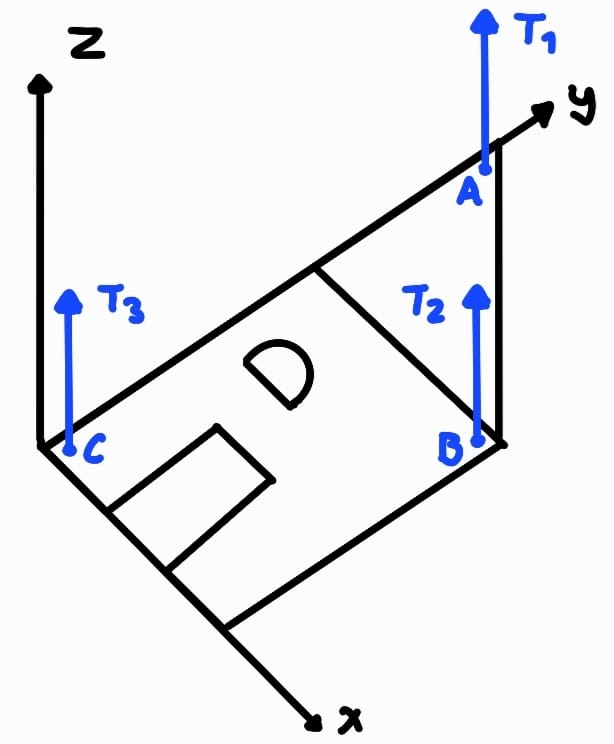
\includegraphics[width=0.3\textwidth]{Sistema_Fuerzas.jpg}
        \caption{Sistema de fuerzas}
    \end{figure}
    Momento aplicado con respecto al origen:
    $$M^{T_1}_O = \bar{OA} \times T_1 = (\hat{i} + 48\hat{j}) \times (1.6383\hat{k}) = 78.6384\hat{i} - 1.6383\hat{j} \unit{[N\cdot cm]}$$
    $$M^{T_2}_O = \bar{OB} \times T_2 = (28\hat{i} + 28\hat{j}) \times (6.5001\hat{k}) = 182.0028\hat{i} - 182.0028\hat{j} \unit{[N\cdot cm]}$$
    $$M^{T_3}_O = \bar{OC} \times T_2 = (0.8\hat{i} + \hat{j}) \times (4.7885\hat{k}) = 4.7885\hat{i} - 3.8308\hat{j} \unit{[N\cdot cm]}$$
    Suma de los tres pares de trasporte:
    $$\sum_{i = 1}^{3} M^T_O = (78.6384 + 182.0028 + 4.7885)\hat{i} - (1.6383 + 182.0028 + 3.8308)\hat{k} $$
    $$\sum_{i = 1}^{3} M^T_O = 265.4297\hat{i} - 187.4719\hat{j} \unit{[N\cdot cm]}$$
    Suma de las tres fuerzas (Resultante R):
    $$\sum_{i = 1}^{3} T_i = R =(1.6383 + 6.5001 + 4.7885)\hat{k} \unit{[N]} = 12.9269\hat{k} \unit{[N]}$$

    \begin{figure}[ht]
        \centering
        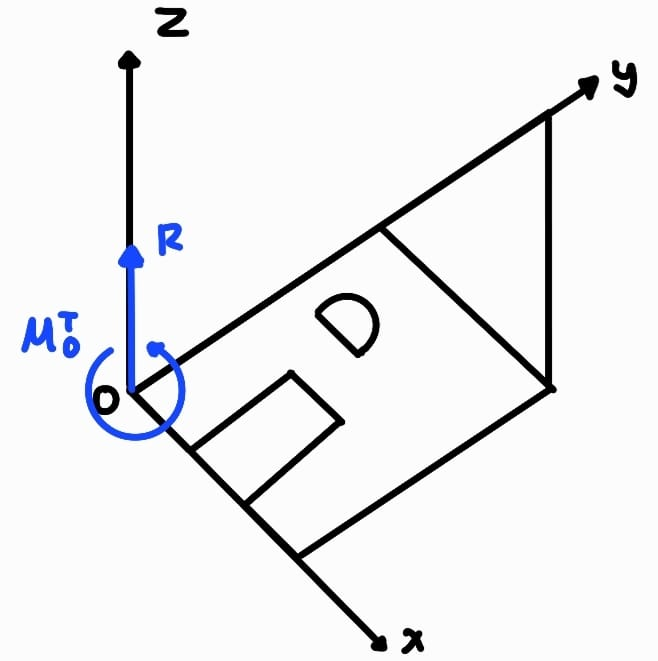
\includegraphics[width=0.3\textwidth]{Sistema_Fuerza-Par.jpg}
        \caption{ Sistema fuerza$-$par aplicado en el origen}
    \end{figure}
    \newpage
    Coordenadas del centro de gravedad ``G'':
    $$\sum_{i=1}^{3} M^T_{O} = M^R_{O}$$
    $$265.4297\hat{i} - 187.4719\hat{j} = \bar{OG} \times (12.9269\hat{k})$$
    $$265.4297\hat{i} - 187.4719\hat{j} = (G_x\hat{i} + G_y\hat{j}) \times (12.9269\hat{k})$$
    $$265.4297\hat{i} - 187.4719\hat{j} =  12.9269G_y\hat{i} - 12.9269G_x\hat{j}$$

    $$- 12.9269G_x\hat{j} = - 187.4719\hat{j}$$
    $$G_x = \frac{- 187.4719\hat{j}}{- 12.9269\hat{j}} = 14.5025 \unit{[cm]}$$

    $$12.9269G_y\hat{i} = 265.4297\hat{i}$$
    $$G_y = \frac{265.4297\hat{i}}{12.9269\hat{i}} = 19.8369 \unit{[cm]}$$

    $$G(14.5025, 19.8369) \unit{[cm]}$$

    \subsection*{Décimo segundo paso}
    Con las coordenadas del centro de gravedad ``G'', obtenidas en el paso anterior se marca con un ``pequeño círculo'' la letra ``G'' en la tabla de madera.

    \begin{figure}[ht]
        \centering
        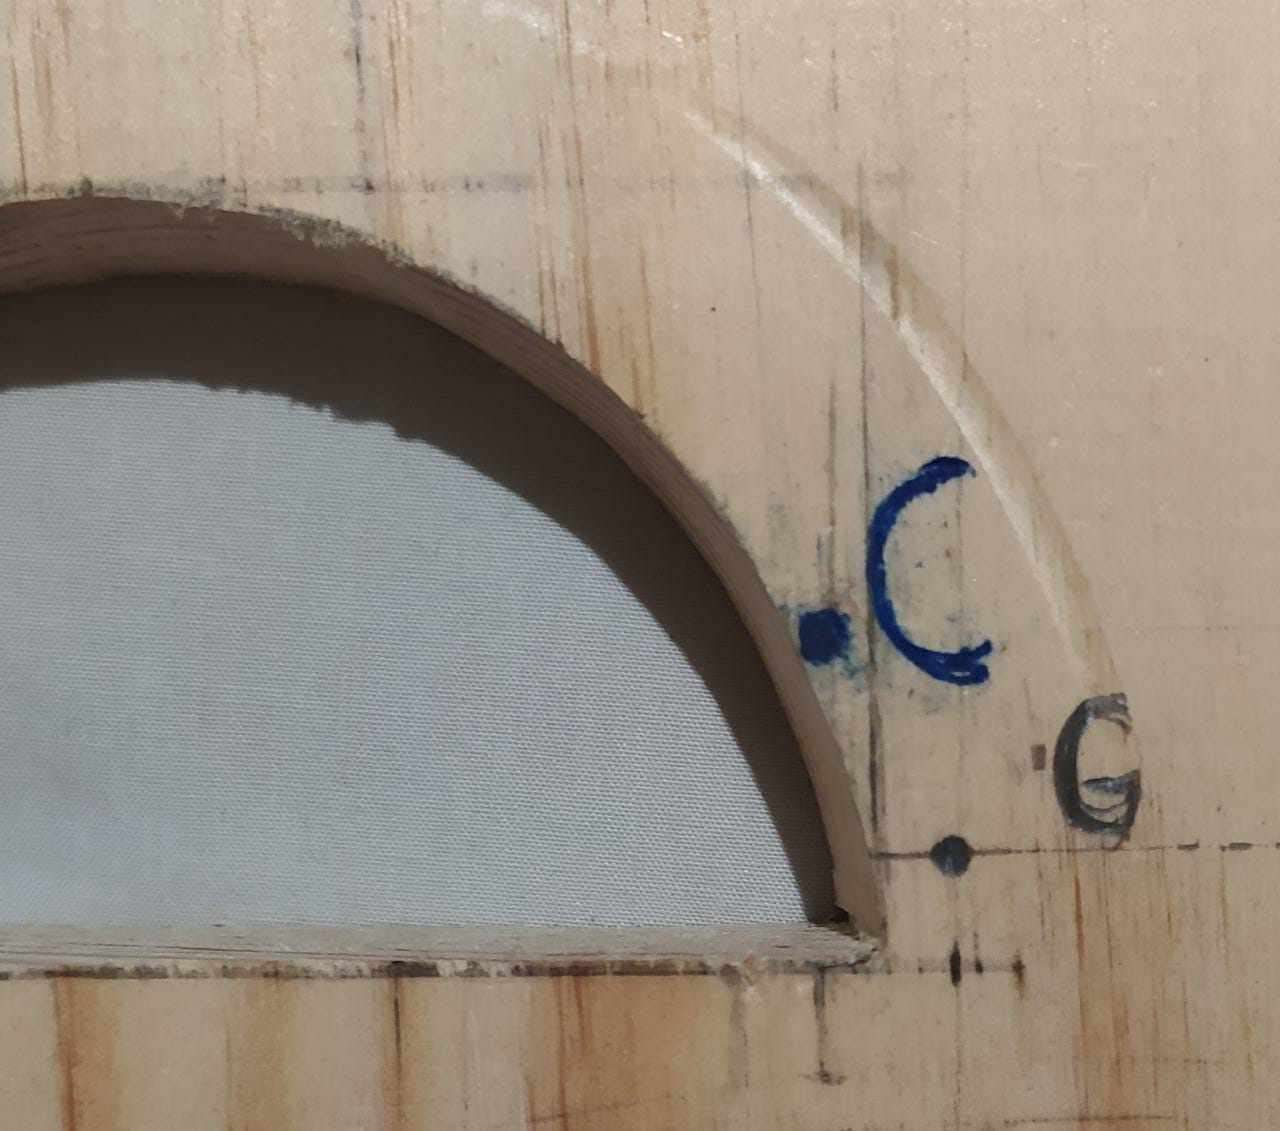
\includegraphics[width=0.5\textwidth]{PuntoG.jpg}
        \caption{Centro de gravedad marcado}
    \end{figure}

    \hfill
    \section{Comprobación de resultados}
    \subsection*{Décimo tercer paso. Comprobación del equilibrio de fuerzas}
    Magnitud del peso de la tabla: 
    $$W=mg=(1.365 \unit{[kg]})(9.78 \unit{m/s^2}) = 13.3497 \unit{[N]}$$
    Resultante de las 3 fuerzas: 
    $$R = 12.9269 \unit{[N]}$$
    Porcentaje de error: 
    $$\%EE=\frac{|W-R|}{W}100\%=\frac{|13.3497 - 12.9269|}{13.3497}100\% = 3.1671\%$$

    \subsection*{Décimo cuarto paso. Comprobación del valor del peso W}
    Volumen de cada figura simple:
    $$V_1 = (A_1 \unit{[cm^2]})(1.8 \unit{[cm]}) = (300 \unit{[cm^2]})(1.8 \unit{[cm]}) = 540 \unit{[cm^3]}$$
    $$V_2 = (A_2 \unit{[cm^2]})(1.8 \unit{[cm]}) = (900 \unit{[cm^2]})(1.8 \unit{[cm]}) = 1620 \unit{[cm^3]}$$
    $$V_3 = (A_3 \unit{[cm^2]})(1.8 \unit{[cm]}) = (-39.27 \unit{[cm^2]})(1.8 \unit{[cm]}) = -70.686 \unit{[cm^3]}$$
    $$V_4 = (A_4 \unit{[cm^2]})(1.8 \unit{[cm]}) = (-60 \unit{[cm^2]})(1.8 \unit{[cm]}) = -108 \unit{[cm^3]}$$
    Volumen total: 
    $$V_{total}=\sum_{i = 1}^{4} V_{i} = 540 + 1620 - 70.686 - 108 \unit{[cm^3]} = 1981.314 \unit{[cm^3]}$$
    Peso específico del triplay (proporcionado por la maderería): 
    $$\gamma =  6686.5221 \unit{[N/m^3]} =  6.6865 \times 10^{-3} \unit{[N/cm^3]}$$
    Volumen total por el peso específico: 
    $$W_{teo}=V_{total}\cdot\gamma = (1981.314 \unit{[cm^3]})(6.6865 \times 10^{-3} \unit{[N/m^3]}) =  13.2481\unit{[N]}$$
    Porcentaje de error: $$\%E=\frac{|W_{teo} - W|}{W_{teo}}100\%=\frac{|13.2481 - 13.3497|}{13.2481}100\% = 0.77 \%$$

    \subsection*{Décimo quinto paso. Comprobación de la ubicación del centro de gravedad de la tabla}
    Coordenadas del centroide: 
    $$C(13.85, 21.23) \unit{[cm]}$$
    Coordenadas del centro de gravedad: 
    $$G(14.5025, 19.8369) \unit{[cm]}$$ 
    Diferencia entre ``C'' y ``G'': 
    $$|x_{C}-x_{G}| \unit{[cm]} = |13.85 - 14.5025| \unit{[cm]} = 0.6525 \unit{[cm]}$$
    $$|y_{C}-y_{G}| \unit{[cm]} = |21.23 - 19.8369| \unit{[cm]} = 1.3931 \unit{[cm]}$$

    \subsection*{Décimo sexto paso. Conclusiones}    
    La búsqueda de la ubicación del centroide ``C'' fue más sencilla por que la figura esta formada por figuras simples, lo hizo que los cálculos fueran satisfactorios. El equilibrio fue muy bueno al sostenerlo con un área circular con un radio de 1 [cm], ya que nuestra figura resultó algo grande y pesada. 

    \begin{wrapfigure}{r}{0.4\textwidth}
        \centering
        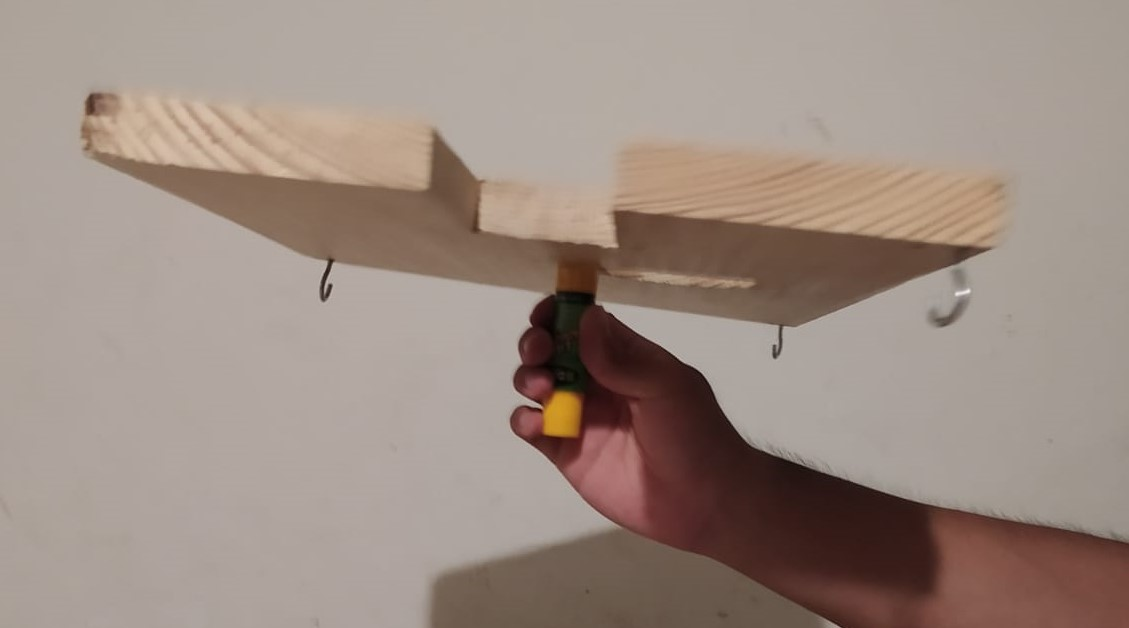
\includegraphics[width=0.3\textwidth]{Equilibrio2.jpg}
        \caption{Punto de apoyo en ``G''}
    \end{wrapfigure}

    Por otro lado, el porcentaje de error del centro de gravedad ``G'' fue sin duda provocado por el error de precisión en las tensiones por parte de nuestro elemento elástico, ya que, a falta de resortes o dinamómetro recurrimos a la ligas las cuales, dados nuestros resultados, probablemente tengan la menor exactitud.
    
    A pesar de eso obtuvimos un error de exactitud de aproximadamente 3\%, lo que nos indica que tanto los cálculos como las mediciones se realizaron lo mas correcto posible. 
    
    Para terminar, logramos conseguir resultados altamente satisfactorios y, con ello, reafirmamos y pusimos en práctica los conocimientos obtenidos en clase a la hora de traerlos a la realidad.
\end{document}